\documentclass[12pt]{article}

% Packages
\usepackage{amsmath, amssymb}
\usepackage{geometry}
\usepackage{graphicx}
\graphicspath{{../../images/}}

\usepackage[colorlinks = true,
            linkcolor = blue,
            urlcolor  = blue,
            citecolor = blue,
            anchorcolor = blue]{hyperref}
\usepackage{enumitem}
\usepackage[backend=biber, style=numeric]{biblatex}
\addbibresource{sba_manifold.bib}
\usepackage[skins]{tcolorbox}
\usepackage{graphicx}
\graphicspath{{../../images/}}
\usepackage[T1]{fontenc}
\usepackage[ttdefault=true]{AnonymousPro}
\renewcommand*\familydefault{\ttdefault} %% Only if the base font of the document is to be typewriter style
% Page setup

\geometry{margin=1in}





\begin{document}

\begin{tcolorbox}[halign=flush center]
         \textbf{Analysis of Risky Borrowers}
   
 \end{tcolorbox}

\section{Introduction}
This article builds upon the \href{https://github.com/rajivsam/descriptive_analytics/blob/main/examples/sba_7a_loans_analysis/sba_7a_loans_desc_analysis.pdf}{bad borrower model with graph features}. While the previous work demonstrated how graph-based features can enhance supervised learning for predicting bad borrowers, this article focuses on leveraging graph-based representations to interpret and apply the results of such prediction models. 

To summarize the key findings from the \emph{bad borrower} prediction model: it successfully screened approximately $80\%$ of the loans, leaving about $20\%$ for further analyst review. When a loan is flagged as \emph{bad} by the model, the next challenge is to interpret this outcome. The approach presented here addresses this by providing a framework for understanding the flagged loans.

Both the \emph{bad borrower prediction} model and this work rely on the concept of a \emph{neighborhood graph} as a central idea. However, while both use graph-based features, the method of featurization and the modeling approach differ. In this article, the focus shifts to an \emph{unsupervised} approach, using a different featurization strategy to construct the neighborhood graph and interpret borrower profiles.


\section{Methodology}
\begin{enumerate}
    \item We focus on borrowers identified as \emph{risky}, specifically those located within the \emph{risky neighborhood region}.
    \item For interpretability, we featurize borrowers using their attributes in the raw data space (after cleaning), rather than the target-encoded features used in the bad borrower model. This approach ensures that similarities are based on demographic and business characteristics (e.g., state, business type), making the resulting clusters more meaningful for analysis.
    \item The dataset contains both categorical (e.g., city, state) and numerical (e.g., loan term, interest rate) attributes. To measure similarity between borrowers with mixed data types, we use the \emph{Gower Similarity} metric \cite{gower1971general}, which produces a pairwise similarity matrix.
    \item Using this similarity matrix, we construct a \emph{neighborhood graph} representing relationships among borrowers. We then apply \emph{spectral clustering} to this graph. Spectral clustering is well-suited for data that may lie on complex, non-linear manifolds, as it leverages the structure of the neighborhood graph rather than relying solely on Euclidean distances. For implementation details, see Section~\ref{sec:clustering} and references \cite{von2007tutorial, stat_ml_spectral_graph_theory}.
    \item For each cluster, we compute the charge-off rate (i.e., the proportion of borrowers in the cluster who defaulted) using a simple group-by operation. This provides a cluster-level measure of risk.
    \item Each risky borrower is assigned to a single cluster. When an analyst reviews a borrower flagged as risky by the prediction model, the risk profile of the borrower's cluster offers interpretable context for the decision.
    \item The spectral clustering process also yields a low-dimensional \emph{manifold} embedding of the borrowers, which can be visualized using techniques such as t-SNE \cite{maaten2008visualizing} to further aid interpretation.
\end{enumerate}
\section{Clustering}\label{sec:clustering}
This section outlines the main concepts and reasoning behind the use of \emph{spectral clustering} in our analysis. For a comprehensive introduction to spectral clustering, refer to \cite{stat_ml_spectral_graph_theory} and the tutorial by von Luxburg \cite{von2007tutorial}. The construction of a \emph{neighborhood graph} is central to our approach, as well as to the \emph{bad borrower prediction} model. This technique is widely used to transform tabular (relational) data into a \emph{homogeneous graph}\footnote{Homogeneous graphs are one of three common analysis patterns in business applications. See \cite{stat_ml_nbrh_graph} for more details.} suitable for graph-based machine learning.

At the heart of spectral clustering lies the \emph{Laplacian} matrix, which is derived from the neighborhood graph and encodes the local connectivity of each node. The eigenvalues and eigenvectors of the Laplacian provide critical information for clustering: specifically, the number of clusters is determined by identifying the \emph{spectral gap }—a significant jump in the sequence of the smallest eigenvalues. The corresponding eigenvectors are then used to embed the data in a lower-dimensional space where standard clustering algorithms, such as $K$-Means, can be applied. The reader interested in the connection between eigenvalues of the Laplacian and thier interpretaion, see \cite{marsden2013eigenvalues}.

In practice, the analyst inspects the first several (e.g., 50) eigenvalues of the Laplacian to locate the spectral gap, which indicates the optimal number of clusters. The number of eigenvectors used in the embedding typically matches the number of clusters. For implementation details—including the construction of the Laplacian and the application of spectral clustering to this dataset—see \href{https://github.com/rajivsam/descriptive_analytics/blob/main/notebooks/sba_cluster_featurization.ipynb}{this notebook}.


\section{Results} \label{sec:results}
The key results from applying \emph{spectral clustering} to the risky neighborhood data is as follows. We start with the identification of the \emph{spectral gap}. The plot of the first $50$ or so eigenvalues is shown in the figure below.
\begin{figure}[h!]
    \centering
    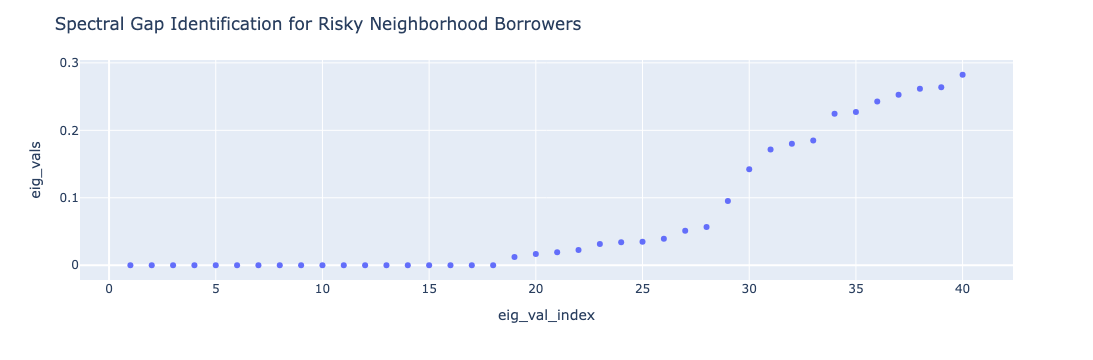
\includegraphics[width=0.7\textwidth]{spectral_gap_identification.png}
    \caption{Spectral gap: Plot of the first 50 eigenvalues of the Laplacian matrix. The distinct jump indicates the optimal number of clusters.}
    \label{fig:spectral_gap}
\end{figure}
The location of the gap can be identified by calculating the difference between succesive eigenvalues and finding the maximum value of the gap. If the maximum gap occurs between values $k$ and $k+1$, we use $k$ as the optimal number of clusters. For the risky neighborhood data, $k$ was $29$. For references and a detailed explaination, please see \cite{von2007tutorial}.

Once the spectral gap is identified, we can generate the embedding and run $K-Means$ clustering with the optimal number of clusters on it. The embedding dimension is generally the same as the number of clusters. The embedding is the representation of the risky neighborhood in the \emph{manifold}. We can then run \emph{tsne} \cite{maaten2008visualizing} to visualize the clusters, this is shown in \ref{fig:tsne_plot}

\begin{figure}[h!]
    \centering
    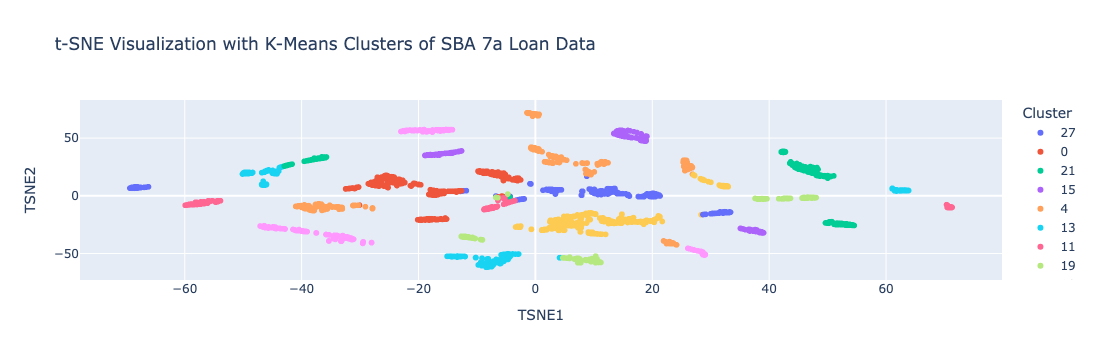
\includegraphics[width=0.7\textwidth]{tsne_plot_visualization.png}
    \caption{t-SNE visualization of risky neighborhood clusters.}
    \label{fig:tsne_plot}
\end{figure}

We now examine key outcomes from the clustering analysis. One important aspect is the distribution of cluster sizes. Spectral clustering aims to produce partitions of comparable size, known as a \emph{balanced cut}. As shown in Figure~\ref{fig:cluster_sizes}, the algorithm achieves a reasonable balance: with approximately $3{,}000$ borrowers in the risky neighborhood, there are no clusters that are disproportionately large or small. 

Figure~\ref{fig:cluster_charge_off_rates} displays the charge-off rates across these clusters. The results indicate that the \emph{risky neighborhood} feature is highly informative—most clusters exhibit elevated charge-off rates. Thus, when a borrower is flagged as \emph{bad} by the classifier, they are assigned to a cluster where the expected charge-off rate is consistently high. This tells the analyst reviewing the decision why the borrower is risky and how risky they are.

\begin{figure}[h!]
    \centering
    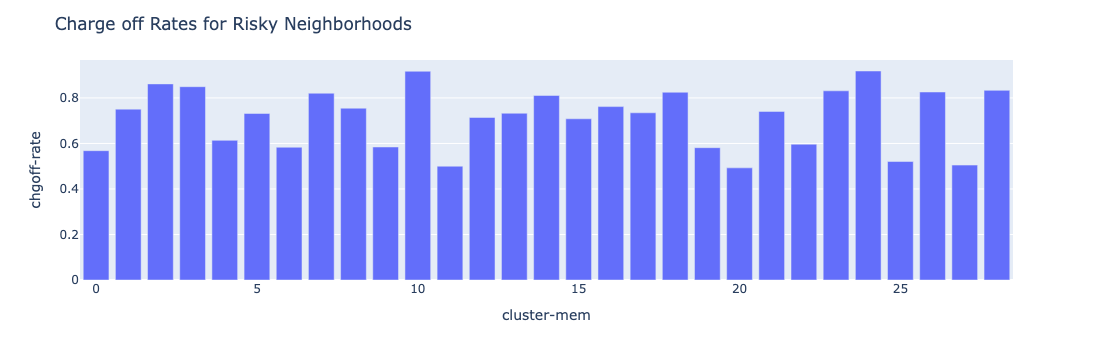
\includegraphics[width=0.7\textwidth]{sba_loans_charge_offs_risky_nbrh.png}
    \caption{Charge off rates in the clusters from risky neighborhood data.}
    \label{fig:cluster_charge_off_rates}
\end{figure}

\begin{figure}[h!]
    \centering
    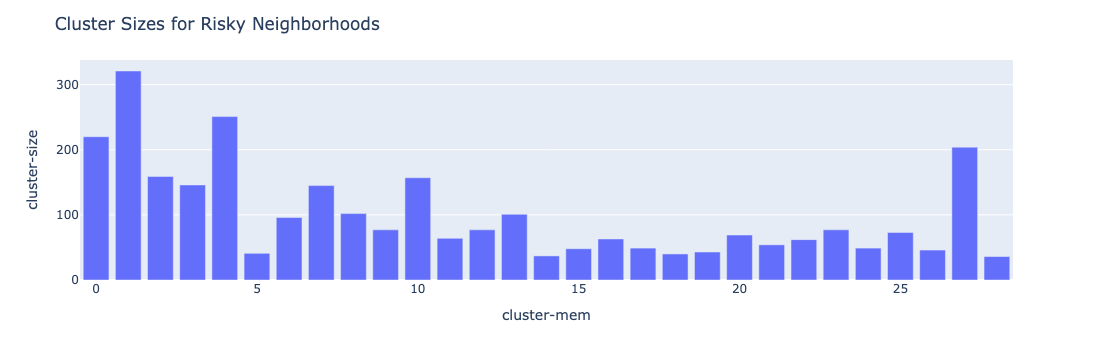
\includegraphics[width=0.7\textwidth]{sba_loans_cluster_sizes.png}
    \caption{Cluster sizes for the risky neighborhood data.}
    \label{fig:cluster_sizes}
\end{figure}

The clustering can have useful applications. Instead of relying on an \emph{average} loss estimate for lending to a risky borrower, assigning borrowers to specific clusters enables a more granular assessment of risk. This finer resolution is particularly valuable for structuring investment products, such as loan portfolios, where risk can be segmented into distinct tranches. By understanding the risk profile at the cluster level, analysts and investors can make more informed decisions and tailor products to different risk appetites. At a loan level, it is also possible to apply frameworks such as \cite{verbraken2012novel} to make cost-benefit based decisions.

\section{Discussion and Insights}
Both this example and the \emph{bad borrower model with graph features} highlight the effectiveness of constructing a \emph{homogeneous graph} from relational data using an appropriate similarity measure. By carefully selecting a similarity or dissimilarity metric tailored to the dataset, one can generate a graph structure that captures meaningful relationships between examples. A central question in this process is: \emph{How should two examples in the dataset be compared?} The answer to this guides the choice of similarity measure and, ultimately, the quality of the resulting graph-based analysis.
A key step in graph-based machine learning is constructing a \emph{vector} representation of the nodes or the graph itself, commonly referred to as an \emph{embedding}. In this work, we employed a \emph{spectral} embedding approach. The choice of embedding technique depends on factors such as the size of the graph and whether the model needs to generalize to previously unseen examples (i.e., whether the setting is transductive or inductive). The relation to graph idea focuses on building a graph from relational data, the process of embedding the graph —transforming it into a form suitable for downstream machine learning tasks requires its own dedicated analysis. Please see \cite{chami_etal}, \cite{hamilton2020graph} for a detailed treatment of approaches to embedding a graph. The reader should be aware that there are other approaches to embedding a graph, such as \emph{random walks} (see \cite{leskovic_jure_cs_224_rw_lecture}). The spectral approach was used here because the size of the problem was amenable to this algorithm. There is also extensive literature on how to apply this algorithm in the wild.
The approach of using one model to predict rare events and another to provide interpretability or context for positive predictions is a common pattern in applied analytics. This paradigm appears in domains such as fraud detection, healthcare interventions for rare diseases, and customer churn analysis. However, it is important to recognize that the choice of features and the method of featurization can vary significantly across applications. As demonstrated by the two SBA loan examples, effective featurization requires careful experimentation and validation in collaboration with domain experts to ensure that the features capture the relevant aspects of the problem.
\printbibliography

\end{document}